\chapter{Exercise 11}
The purpose of the exercise is to understand the theory behind
parametric curves and surfaces and how to use this theory to create
geometric models. The theory includes Bezier, uniform B-spline,
non-uniform B-spline and NURBS (non-uniform rational B-spline)
curves and surfaces.

\section{Part 1}
Following instructions in the exercise I obtained a program drawing bezier
curves which is shown in the figure \ref{fig:exercise_11_part_1}.
\begin{figure}[ht!]
	\begin{center}
		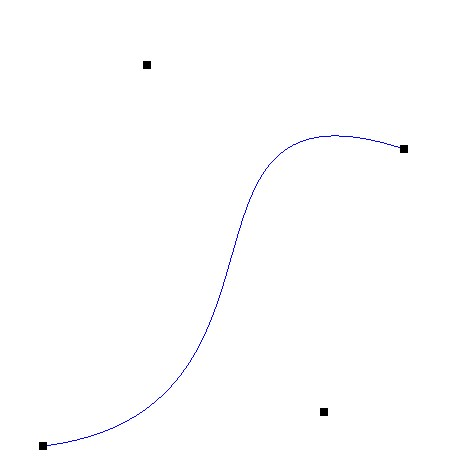
\includegraphics[width=.6\textwidth]{figures/exercise_11_part_1}
	\end{center}
	\vspace{-4.5ex}\caption{Exercise 11 part 1}
	\label{fig:exercise_11_part_1} 
\end{figure}

\section{Part 2}
Following instructions in the exercise I succeeded in drawing a circle
which is shown in the figure \ref{fig:exercise_11_part_2}.
\begin{figure}[ht!]
	\begin{center}
		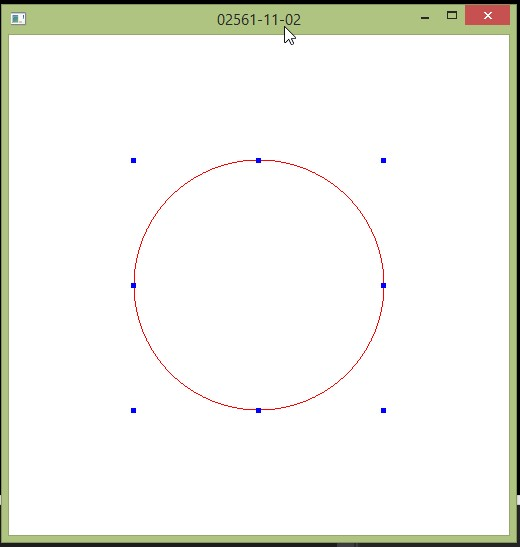
\includegraphics[width=.6\textwidth]{figures/exercise_11_part_2}
	\end{center}
	\vspace{-4.5ex}\caption{Exercise 11 part 2}
	\label{fig:exercise_11_part_2} 
\end{figure}

\section{Part 3}
Below we can see results for 4 modes I had to implement:
\begin{enumerate}
\item Bezier - figure \ref{fig:exercise_11_part_3_1}
\item Uniform B-Spline \ref{fig:exercise_11_part_3_2}
\item Non-uniform B-Spline \ref{fig:exercise_11_part_3_3}
\item NURBS (Non-Uniform Rational B-Spline) \ref{fig:exercise_11_part_3_4}
\end{enumerate}
\begin{figure}[ht!]
	\begin{center}
		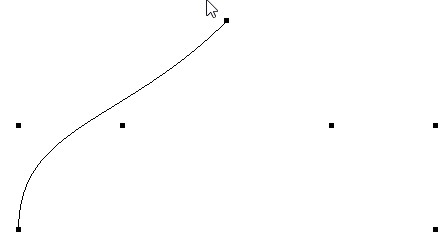
\includegraphics[width=1.0\textwidth]{figures/exercise_11_part_3_1}
	\end{center}
	\vspace{-4.5ex}\caption{Exercise 11 part 3 bezier}
	\label{fig:exercise_11_part_3_1} 
\end{figure}
\begin{figure}[ht!]
	\begin{center}
		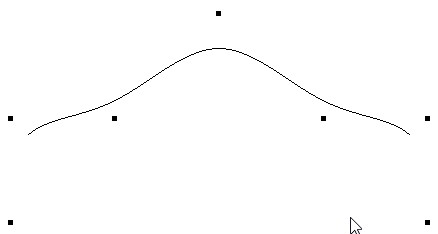
\includegraphics[width=1.0\textwidth]{figures/exercise_11_part_3_2}
	\end{center}
	\vspace{-4.5ex}\caption{Exercise 11 part 3 uniform b-splines}
	\label{fig:exercise_11_part_3_2} 
\end{figure}
\begin{figure}[ht!]
	\begin{center}
		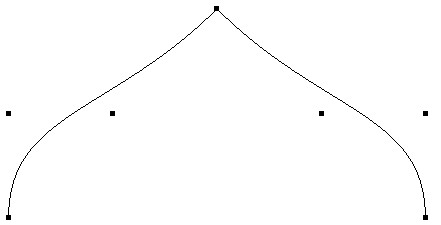
\includegraphics[width=1.0\textwidth]{figures/exercise_11_part_3_3}
	\end{center}
	\vspace{-4.5ex}\caption{Exercise 11 part 3 non-uniform b-splines}
	\label{fig:exercise_11_part_3_3} 
\end{figure}
\begin{figure}[ht!]
	\begin{center}
		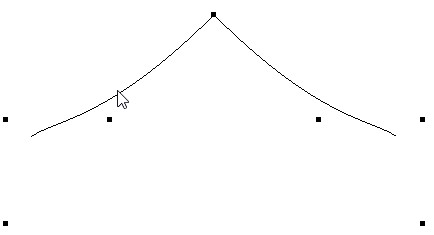
\includegraphics[width=1.0\textwidth]{figures/exercise_11_part_3_4}
	\end{center}
	\vspace{-4.5ex}\caption{Exercise 11 part 3 NURBS}
	\label{fig:exercise_11_part_3_4} 
\end{figure}
\clearpage
\section{Part 4}
By use of code in the listing \ref{lst:non_uni_surf_code} I managed to get result shown in the figure \ref{fig:exercise_11_part_4}.
\begin{lstlisting}[language=cpp, caption={3D non uniform b-spline surface}, label={lst:non_uni_surf_code}]
const int numberOfControlPointsU = 7;
const int numberOfControlPointsV = 7;
vec3 controlPointsU[numberOfControlPointsU] = {vec3(-10.,0.,0.),
	vec3(-5.,-5.,0.),vec3(-2.,-5.,0.),vec3(0.,0.,0.),
	vec3(2.,5.,0.),vec3(5.,5.,0.),vec3(10.,0.,0.)};

vec3 controlPointsV[numberOfControlPointsV] = { vec3(0.,0.,0.),
	vec3(0.,1.,0.),vec3(0.,1.,0.),vec3(0.,0.,0.),
	vec3(3.,0.,0.),vec3(3.,0.,0.),vec3(0.,0.,0.)};
	
vec3 controlPointsSurface[numberOfControlPointsU][numberOfControlPointsV];

void init_surface(){
   int u, v;
   for (u = 0; u < numberOfControlPointsU; u++){
	   for (v = 0; v < numberOfControlPointsV;v++){
		   float x = controlPointsU[u].x;
		   float y = controlPointsU[u].y;
		   controlPointsSurface[u][v].x = x;
		   controlPointsSurface[u][v].y = x >= 0 ? y * controlPointsV[v].x : y * controlPointsV[v].y;
		   controlPointsSurface[u][v].z = ((float)v/7.0f - 0.5f)*30;
	   }}}  
\end{lstlisting}
\begin{figure}[ht!]
	\begin{center}
		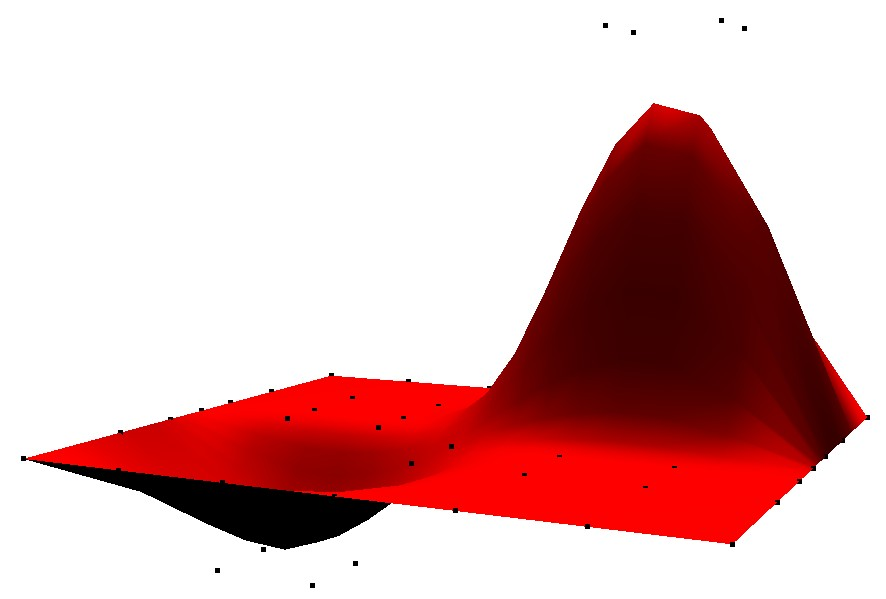
\includegraphics[width=1.0\textwidth]{figures/exercise_11_part_4}
	\end{center}
	\vspace{-4.5ex}\caption{Exercise 11 part 4}
	\label{fig:exercise_11_part_4} 
\end{figure}
